%-----------------------------------------------------------------------------------------
%  Dieses Projekt wurde erstellt mit der LaTeX Vorlage von Jonas Bingel
%  Die LaTeX Vorlage kann heruntergeladen werden unter: github.com/JonasBingel/HSMZ-Thesis-Template
% -----------------------------------------------------------------------------------------

% Erklärender Text zu dieser Datei --------------------------------------------------------
% Die Datei Arbeit.tex ist die Hauptdatei, die dem LaTeX-Kompiler übergeben wird.
% Diese Datei ist zu verwenden, wenn die eigentliche Haus/Bachelor/Masterarbeit erstellt werden soll.
% In dieser Datei wird
%  - das Dokument erstellt und alle anderen tex-Dateien werden geladen.
%  - die .bib-Datei eingebunden zur Bereitstellung der Quellen
%  - die Struktur des Dokuments wird definiert
% -----------------------------------------------------------------------------------------

\documentclass[
% ngerman, % neue Deutsche Rechtschreibung
headings=normal, % normale Headings
captions=tableheading, % Positioniert Captions über Tabellen
listof=totoc,
bibliography=totoc,
%usegeometry, % Auskommentieren wenn Package geometery verwendet wird
overfullrule, % entfernen nach abschluss der bearbeitung
% Default Values, die scrreprt nutzt
oneside, % Einseitige Seitengenerierung
12pt, % Font size
a4paper, % paper
]{scrreprt}
\linespread{1.5}
\KOMAoptions{%
  DIV=12,
  parskip=half*,
% %BCOR=korrektur, % absoluter Wert der Bindekorrektur
}

% Erklärender Text zu dieser Datei --------------------------------------------------------
% Die Datei Metadaten.tex dient der Definition von Metadaten zur vorliegenden Arbeit.
% Dies umfasst Informationen zu
%  - der Arbeit selbst(Titel, Art)
%  - dem Betreuer
%  - dem Hochschule
%  - ggf. kooperierenden Unternehmen
% Die Metadaten werden genutzt in Titelseite.tex, Sperrvermerk.tex und Erklaerung.tex
% Ferner werden die Metadaten des exportierten PDFs entsprechend gesetzt - eine Konfiguration ist in Packages.tex möglich.
% -----------------------------------------------------------------------------------------

% Meta-Daten zu dieser Arbeit ------------------------------------------------------------
\newcommand{\art}{Masterarbeit\xspace}
\newcommand{\titel}{Sensorama: A task-specific Telepresence Application for Contemporary Dance\xspace}
\newcommand{\hochschule}{Hochschule Mainz}
\newcommand{\hochschulezusatz}{University of Applied Sciences}
\newcommand{\logo}{logo_hsmz.png}
\newcommand{\fachbereich}{Technik}
\newcommand{\studiengang}{Geoinformatik und Vermessung}
\newcommand{\akadGrad}{Master of Engineering}

\newcommand{\autor}{Vorname Nachname}
\newcommand{\strasseAutor}{Straße}
\newcommand{\stadtAutor}{PLZ Ort}
\newcommand{\matrikelnr}{123456}

\newcommand{\unternehmen}{Unternehmen}
\newcommand{\datumAblaufSperrvermerk}{01.01.1970}

\newcommand{\betreuer}{Prof. Dr. Betreuer}
\newcommand{\datumAbgabe}{01.01.1970}
\newcommand{\ort}{Mainz}


% Erklärender Text zu dieser Datei --------------------------------------------------------
% Die Datei Packages.tex dient als zentrale Datei, in der alle genutzten Packages geladen und konfiguriert werden.
% Basierend auf den Anforderungen sind ggf. Konfigurationen vereinzelt zu ändern - entsprechende Stellen sind mit %TODO gekennzeichnet.
% Beispiele für solche Anforderungen sind
%  - Package biblatex: Definition, des Zitationsstils und Aufbau des Literaturverzeichnisses; Default ist IEEE, Konfiguration für APA ist hinterlegt
%  - Package minted: Definition, wie Source Code von Sprachen dargestellt werden soll
%  - Zur korrekten Darstellung des Inhaltsverzeichnisses die "breiteste" Seitenzahl angeben
%
% HINWEIS: Die Reihenfolge, in der Packages geladen werden ist wichtig. Hinweise aus den Dokumentationen der einzelnen Packages sind daher unbedingt zur berücksichtigen, wenn weitere Packages aufgenommen werden sollen.
% -----------------------------------------------------------------------------------------
% \usepackage[a4paper, top=2.5cm]{geometry}
\usepackage[utf8]{inputenc}
\usepackage[T1]{fontenc}
\usepackage[UKenglish]{babel}
\usepackage{lmodern}
\usepackage{fancyhdr}
\usepackage{xspace} % Leerzeichen hinter parameterlosen Makros nicht als Endzeichen interpretieren
\usepackage{graphicx} %Abbildungen
\usepackage{pdfpages} %Einfügen von PDF-Seiten
\includepdfset{scale=0.7, frame, pagecommand={\thispagestyle{plain}}}
\graphicspath{{04_Artefakte/01_Abbildungen/}}
\usepackage{caption} % Bildunterschriften
\usepackage{subcaption} % https://www.ctan.org/pkg/subcaption

\usepackage{tabularx} % Tabellen
\usepackage{booktabs} % Bessere Tabellen
\usepackage[longtable]{multirow}
\usepackage{longtable}

\usepackage{amsmath}
\usepackage{amsfonts}
\usepackage{bbm}

\usepackage{xcolor}
%\usepackage{chngcntr} % fortlaufende Nummerierung von Fußnoten

\usepackage[colorinlistoftodos]{todonotes} % to disable todos use option disable, alternatively use obeyDraft or obeyFinal
\usepackage{blindtext}

\usepackage{microtype} % auskommentieren moeglich, wenn Typografie nicht zufriedenstellend

\usepackage[bottom]{footmisc} % https://golatex.de/viewtopic.php?f=21&t=24052
% Verlinkung und PDF Bookmarks https://tex.stackexchange.com/a/83051
\usepackage[nospace]{varioref}
% extensions keep all links black, only urls are blue: https://tex.stackexchange.com/a/401885/220502
\usepackage[hidelinks, colorlinks, allcolors=., urlcolor=blue]{hyperref}
\usepackage{bookmark}
\hypersetup{
    pdftitle={\titel},
    pdfauthor={\autor},
    pdfcreator={\autor},
    pdfsubject={\titel},
    pdfkeywords={\titel},
}
\usepackage{cleveref}

% Literaturverzeichnis und Quellenverwaltung mittels biblatex
%TODO Änderungen des Zitationsstils und Literaturverzeichnisses
% Zitationsstil hier auswählen:

\newcommand{\ZitatStil}{apa} % (apa oder ieee)

\ifthenelse{\equal{\ZitatStil}{apa}}{%
  \usepackage[sortlocale=auto,sorting=nyt,style=apa]{biblatex}%
}{
\ifthenelse{\equal{\ZitatStil}{iee}}{%
  \usepackage[backend=biber,style=ieee,dashed=false,]{biblatex}%
}}


% Verwalten von Abkuerzungen und einem Abkuerzungsverzeichnis
\usepackage[printonlyused]{acronym} % https://www.ctan.org/pkg/acronym

% Packages for forcing floats https://robjhyndman.com/hyndsight/latex-floats/
\usepackage{afterpage}
\usepackage[section]{placeins}
\usepackage{censor}


% Erstellen eines Symbolverzeichnisses
\usepackage[intoc, german, stdsubgroups]{nomencl} % https://www.ctan.org/pkg/nomencl
\usepackage{siunitx}
\newcommand{\nomunit}[1]{%
    \renewcommand{\nomentryend}{\hspace*{\fill}\si{#1}}}
\makenomenclature

%TODO Definition der Darstellung von Source Code
\usepackage[newfloat, cache]{minted} % https://www.ctan.org/pkg/minted
\SetupFloatingEnvironment{listing}{name=Listing, placement=b}
\SetupFloatingEnvironment{listing}{listname={Listingverzeichnis}}
\setminted[java]{linenos, fontsize=\footnotesize, frame=lines, breaklines, breakbefore={.}}
\setminted[js]{linenos, fontsize=\footnotesize, frame=lines, breaklines, breakbefore={.}}
\setminted[json]{linenos, fontsize=\footnotesize, frame=lines, breaklines, breakbefore={.}}
\usemintedstyle{friendly}
% new environment for listings longer than one page; https://tex.stackexchange.com/a/53540
\newenvironment{longlisting}{\captionsetup{type=listing}}{}
\usepackage{csquotes}


% Darstellung von Algorithmen und Pseudocode
% do NOT use option naturalnames if you compile with pdflatex and use hyperref
\usepackage[linesnumbered, commentsnumbered, ruled]{algorithm2e} 
\renewcommand{\listalgorithmcfname}{Algorithmusverzeichnis}
\addtotoclist[float]{loa}
\renewcommand\listofalgorithms{\listoftoc[{\listalgorithmcfname}]{loa}}
%\SetAlFnt{\small \normalfont \sffamily} 
\SetAlFnt{\footnotesize} 


% Erstellung neuer Verzeichnisse; Code weitgehend von Markus Kohm und komascript.de 
\DeclareNewTOC[%
  owner=anhang,
  listname={Appendix Listing},% Titel des Verzeichnisses
]{atoc}

\DeclareNewTOC[%
  type=equation,
  listname={Formelverzeichnis},
  tocentrynumwidth=2.3em,
]{loe}

\makeatletter
\renewcommand\@pnumwidth{2em} % vermeiden von overful hbox im Inhaltsverzeichnis

\AfterTOCHead[atoc]{\let\if@dynlist\if@tocleft}
\newcommand*{\useappendixtocs}{%
  \renewcommand*{\ext@toc}{atoc}%
  \scr@ifundefinedorrelax{hypersetup}{}{% damit es auch ohne hyperref funktioniert
    \hypersetup{bookmarkstype=atoc}%
  }%
}
\newcommand*{\usestandardtocs}{%
  \renewcommand*{\ext@toc}{toc}%
  \scr@ifundefinedorrelax{hypersetup}{}{% damit es auch ohne hyperref funktioniert
    \hypersetup{bookmarkstype=toc}%
  }%
  \renewcommand*{\ext@figure}{lof}%
  \renewcommand*{\ext@table}{lot}%
}
\scr@ifundefinedorrelax{ext@toc}{%
  \newcommand*{\ext@toc}{toc}
  \renewcommand{\addtocentrydefault}[3]{%
    \expandafter\tocbasic@addxcontentsline\expandafter{\ext@toc}{#1}{#2}{#3}%
  }
}{}
\newcommand*{\@currententry}{}
% Zwei amsmath-Anweisungen ändern:
\g@addto@macro\make@display@tag{\set@currententry}%
\def\tagform@#1{\maketag@@@{(\ignorespaces#1\unskip\@@italiccorr)}%
  \set@currententry}
\newcommand*{\set@currententry}{%
  \typeout{set current entry}%
  \ifx\@currententry\@empty\else
    \addcontentsline{loe}{equation}{\protect\numberline{\@currentlabel}%
      \@currententry}%
    \global\let\@currententry\@empty
  \fi
}
% Neue Benutzeranweisung
\newcommand*{\equationentry}[1]{%
  \gdef\@currententry{#1}%
}

\makeatother

\usepackage{xpatch}
\xapptocmd\appendix{%
  \useappendixtocs
  \pdfbookmark{Appendix}{appendix}
  \listofatocs
  \addcontentsline{toc}{chapter}{Appendix}
  \bookmarksetupnext{level=-1}
}{}{}

% Pakete, die fuer Informatik Sinn ergeben koennten
% \usepackage{bytefield} % illustration of fields of data https://www.ctan.org/pkg/bytefield


% Uebersetzung fuer Eintraege im Abkuerzungsverzeichnis - Code uebernommen von https://tex.stackexchange.com/a/135507
\makeatletter
\newcommand{\acroforeign}[1]{}

% patch the environment to print the foreign definition:
\AtBeginEnvironment{acronym}{%
  \def\acroforeign#1{ (#1)}%
}

% patch the acronym definition to safe the foreign definition:
\expandafter\patchcmd\csname AC@\AC@prefix{}@acro\endcsname
  {\begingroup}
  {\begingroup\def\acroforeign##1{\csdef{ac@#1@foreign}{##1, }}}
  {}
  {\fail}

% %   renew the first output to include the foreign definition if given:
\renewcommand*{\@acf}[2][\AC@linebreakpenalty]{%
  \ifAC@footnote
    \acsfont{\csname ac@#2@foreign\endcsname\AC@acs{#2}}%
    \footnote{\AC@placelabel{#2}\AC@acl{#2}{}}%
  \else
    \acffont{%
      \AC@placelabel{#2}\AC@acl{#2}%
      \nolinebreak[#1] %
      \acfsfont{(\acsfont{\csname ac@#2@foreign\endcsname\AC@acs{#2}})}%
    }%
  \fi
  \ifAC@starred\else\AC@logged{#2}\fi
}
\makeatother

% Adjusting the width that is reserved for the  pagenumber in listings
% https://projekte.dante.de/DanteFAQ/Verzeichnisse#2
% https://de.comp.text.tex.narkive.com/fAP3Znev/overfull-hbox-im-inhaltsverzeichnis
\makeatletter
\AtBeginDocument{
\newlength{\mylen}
\setlength{\mylen}{\widthof{XVIII}} %TODO hier Text eintragen, der der breitesten Seitennummer im Inhaltsverzeichnis oder einem der anderne Verzeichnisse entspricht
\renewcommand*\@pnumwidth{\the\mylen}
}
\makeatother

\input{00_Allgemein/Befehle}

% Typesetting options
\widowpenalty=10000     % Hurenkinder
\clubpenalty=10000      % Schusterjungen



\addbibresource{sample.bib}
% Wegen dem folgenden Befehl werden im Literaturverzeichnis alle Quellen gelistet, die in der .bib Datei enthalten sind.
% Wird der Befehl entfernt, werden nur die Quellen gelistet, die auch zitiert werden.
% Der Befehl sollte bei Abgabe der Bachelorarbeit entfernt werden.
\nocite{*}
\newcounter{romanConsecutive}

% Set ToC depth to subsubsection
% \setcounter{tocdepth}{4}
% \setcounter{secnumdepth}{4}

\begin{document}
\include{00_Allgemein/ToDo}

\pagestyle{empty}
\renewcommand*{\chapterpagestyle}{empty}
% Erklärender Text zu dieser Datei --------------------------------------------------------
% Die Datei 02_Titelseite.tex dient der Definition der Titelseite.
% Alle Angaben auf der Titelseite werden mit Informationen aus Metadaten.tex gefüllt
% Solange das Design der Titelseite nicht angepasst werden soll, sind in dieser Datei keine manuellen Änderungen notwendig.
% -----------------------------------------------------------------------------------------
\begin{titlepage}

\begin{minipage}{\textwidth}
		\noindent \hfill \includegraphics{\logo}
\end{minipage}
\vspace{6em}

\begin{center}
    {\huge \art}
    
    {\Large zur Erlangung des akademischen Grades \akadGrad}\\
    {\Large im Studiengang \studiengang}
    
    \vspace{3em}
    
    \textbf{{\Large \titel}}
    
    \vspace{3em}
    
    \hochschule \\
    Fachbereich \fachbereich
    
    \vspace{4em}

	\begin{minipage}{\textwidth}
		\begin{tabbing}
		
		Vorgelegt von:  \hspace*{2em}\= \autor \\
		\> \strasseAutor \\
        \> \stadtAutor \\
        \> Matrikel-Nr. \matrikelnr \\
        Betreut von: \> \betreuer \\
        Eingereicht am: \> \datumAbgabe
		\end{tabbing}

	\end{minipage}
\end{center}
\end{titlepage}
% Erklärender Text zu dieser Datei --------------------------------------------------------
% Die Datei 03_Erklaerung.tex dient der Definition der Eidesstattlichen Erklärung.
% Die Datei enthält den Text, der im Leitfaden der Hochschule Mainz vorgegeben ist.
% Wenn ein Bild einer Unterschrift eingefügt werden soll, ist an der Stelle %TODO dem Hinweis zu folgen.
% -----------------------------------------------------------------------------------------
\pdfbookmark{Erklärung}{erklaerung}
\addchap*{Erklärung}
Hiermit erkläre ich, dass ich die vorliegende Masterarbeit
\begin{quote}
\textbf{\titel}   
\end{quote}

selbstständig und ohne fremde Hilfe angefertigt habe. 
Ich habe dabei nur die in der Arbeit angegebenen Quellen und Hilfsmittel benutzt.

Zudem versichere ich, dass ich weder diese noch inhaltlich verwandte Arbeiten als Prüfungsleistung in anderen Fächern eingereicht habe oder einreichen werde.

\vspace{3em}
%TODO Wenn eine Unterschrift eingefügt werden soll, muss nachfolgender Kommentar eingefügt werden
% Einfuegen der Unterschrift als Datei "signature.png", Scale muss ggf. angepasst werden
% \begin{figure}[h]
%     \hspace{9cm}
%     \includegraphics[scale=0.2]{04_Artefakte/01_Abbildungen/signature.png}
% \end{figure}
\ort, den \datumAbgabe \hfill \autor 


\pdfbookmark{Abstract}{abstract}
\addchap*{Abstract}

This study investigates the feasibility of creating a fully customised and task-specific telepresence application based exclusively on open web standards and free software for use in contemporary dance practice.
It surveys existing technologies and paradigms and establishes a practical reference implementation to evaluate its basic functionality and the development process.
The study concludes with a positive assessment of the existing technological landscape and the feasibility to produce task-specific web applications as an intrinsic component in a smaller interdisciplinary projects with a strong focus on digital practice.

Keywords: open-source software, telepresence, contemporary dance, motion capture
 
 Die vorliegende Studie untersucht die Machbarkeit der Entwicklung einer aufgabenspezifischen Telepräsenzanwendung, ausschließlich auf offenen Webstandards und freier Software basierend, für den Einsatz in der zeitgenössischen Tanzpraxis.
 Es wird ein Überblick über existente Technologien und Paradigmen erabeitet und eine Referenzimplementierung erstellt, deren grundlegende Funktionalität evaluiert und der Prozess ihrer Entwicklung bewertet wird.
 Die Studie schließt mit einer positiven Beurteilung, sowohl im Hinblick auf die generelle technologische Landschaft, als auch die Machbarkeit einer aufgabenspezifischen Softwareimplementierung als intrinsischer Komponente von kleineren interdisziplinären Projekten mit einem starken Fokus auf digitaler Praxis.
 

\pagestyle{fancy}
\fancyhf{}
\fancyheadoffset{0cm}
\renewcommand{\headrulewidth}{0pt} 
\renewcommand{\footrulewidth}{0pt}
\fancyhead[R]{\thepage}
\fancypagestyle{plain}{
  \fancyhf{}
  \fancyhead[R]{\thepage}
}
% \pagestyle{plain}
\renewcommand*{\chapterpagestyle}{fancy}
\pagenumbering{Roman}
% Erklärender Text zu dieser Datei --------------------------------------------------------
% Die Datei 05_Verzeichnisse.tex dient der Definition der zu generierenden Verzeichnisse und deren Reihenfolge.
% Wenn einzelne Verzeichnisse nicht generiert werden sollen, sind die entsprechenden Anweisungen auszukommentieren.
% -----------------------------------------------------------------------------------------

% Inhaltsverzeichnis ----------------------------------------------------------------------
\pdfbookmark{Table of contents}{toc}
\tableofcontents

% Abbildungsverzeichnis -------------------------------------------------------------------
\listoffigures

% Tabellenverzeichnis ---------------------------------------------------------------------
% \listoftables

% Abkuerzungsverzeichnis ------------------------------------------------------------------

\newcommand{\abksvz}{List of abbreviations}
\chapter*{\abksvz}
\addchaptertocentry{}{\abksvz}
% Erklärender Text zu dieser Datei --------------------------------------------------------
% Die Datei 06_Abkuerzungen.tex dient der Definition von Abkürzungen, die im Abkürzungsverzeichnis gelistet werden sollen.
% Zur besseren Übersichtlichkeit wird empfohlen die Abkürzungen zentral in dieser Datei zu definieren.
%
% Abkürzungen müssen erst definiert werden mittels \acro bevor diese im eigentlichen Textteil mit \ac verwendet werden können.
% Die Angabe von Übersetzungen zu Abkürzungen ist möglich mittels der Anweisung \acroforeign.
% -----------------------------------------------------------------------------------------
\begin{acronym}
	\acro{3D}{3-dimensional}
	\acro{AJAX}{Asynchronous JavaScript and XML}
	\acro{API}{Application Programming Interface}
	\acro{AR}{Augmented Reality}
	\acro{CLI}{Command-line interface}
	\acro{CPU}{Central Processing Unit}
	\acro{CNCF}{Cloud Native Computing Foundation}
	\acro{CSS}{Cascading Style Sheets}
	\acro{DIY}{Do It Yourself}
	\acro{ES6}{ECMAScript 6}
	\acro{HTML}{HyperText Markup Language}
	\acro{HTTP}{Hypertext Transmission Protocol}
	\acro{IETF}{Internet Engineering Task Force}
	\acro{I/O}{Input/Output}
	\acro{JSX}{JavaScript XML}
	\acro{JS}{JavaScript}
	\acro{NPM}{Node Package Manager}
	\acro{OCI}{Open Container Initiative}
	\acro{PWA}{Progressive Web Application}
	\acro{RFC}{Request For Comments}
	\acro{RTC}{Real-time Communication}
	\acro{SFU}{Selective Forwarding Unit}
	\acro{SPA}{Single Page Application}
	\acro{TCP}{Transfer Control Protocol}
	\acro{TS}{TypeScript}
	\acro{UDP}{User Datagram Protocol}
	\acro{UI}{User Interface}
	\acro{VR}{Virtual Reality}
	\acro{W3C}{World Wide Web Consortium}
	\acro{WebRTC}{Web Real-Time Communication}
	\acro{WebXR}{Web Mixed Reality}
	\acro{XML}{Extensible Markup Language}
	\acro{XR}{Mixed Reality}
\end{acronym}


% Symbolverzeichnis -----------------------------------------------------------------------
% \printnomenclature

% Formelverzeichnis -----------------------------------------------------------------------
% \listofequations

% Listingverzeichnis ----------------------------------------------------------------------
% \listoflistings

% Algorithmenverzeichnis ------------------------------------------------------------------
% \listofalgorithms

\include{00_Allgemein/Nomenklatur}

\setcounter{romanConsecutive}{\value{page}}
\pagenumbering{arabic}
\chapter{Introduction}
\label{chapter:introduction}

\section{Background}

Remote collaboration has become increasingly prevalent in various professional environments through broader digitalisation efforts and significantly accelerated during the COVID-19 pandemic.
As a result, teleconferencing and telepresence platforms that were initially used primarily for international business relations are now much more common in many work environments.
These technologies allow people to work together remotely in real time, usually focusing on streaming video and audio, document sharing and collaborative whiteboarding.
While this covers most use cases in desk-based workplaces, it lacks the immersive qualities required for practices such as contemporary dance, where people relate to physical presence and shared space.
This became apparent in March 2020, when dancers could no longer rehearse and work together due to the lockdown.
Despite this, there were attempts at using videoconferencing to stream and record collaborative rehearsals or dance classes.
Still, these were confined to a screen-centric interface and limited to audio and video.

While commercial conferencing tools dominate in popularity among conferencing applications \parencite{mostPopularConferencingPlatforms}, there are several free and open-source alternatives.
However, these all focus on the most basic form of screen-based conferencing.
Various domain-specific solutions for specialised applications, mainly in telemedicine, industry and the military, support more immersive remote collaboration. Still, these are task-specific and difficult to afford for smaller creative or artistic project setups.

Support for web standards is driven by key industry players \parencite{pushingInteroperabilityForward}, making a wide range of basic functionality accessible in web browsers, as well as access to display and sensor technology and cross-platform deployment on desktop and mobile devices.
This development now provides an increased potential for smaller and more task-specific applications to be built and deployed relatively quickly.
It opens up new possibilities for niche cases of remote collaboration, such as dance practice, where the collaborative agency could be extended from a composite of video streams to the creation of shared virtual environments that facilitate a more personal form of mediating a sense of shared presence.

The standard for \ac{RTC} in Browsers or \ac{WebRTC} \parencite{webRtcSpec} was first proposed by Google in 2011 and became an official \ac{W3C} standard in 2021 \parencite{webRtcOfficialWebStandard}.
It has become the basis for numerous applications, such as some of the conferencing tools mentioned above, media streaming servers such as Wowza or Ant, or real-time frameworks and servers such as Mediasoup, Janus or LiveKit.
In its most basic form, \ac{WebRTC} establishes peer-to-peer connections between devices, allowing low-latency exchange of media streams and arbitrary messages over data channels. However, it can accommodate other more complex and versatile scenarios.

\section{Proposal}

The proposed study examines the feasibility of creating a customised telepresence experience that explicitly covers a specific task not provided by common platforms or products.
A potential target audience for such an application would be tiny and hardly warrants a commercial strategy of external product development, marketing and support.
Extensive software development budgets are also rare in funding schemes supporting smaller cultural production endeavours, and it is relatively common for practitioners themselves to dabble in experimental development or to have a creative coder on the team.
To keep the budgetary requirements for such an implementation at a minimum, relying on open standards and non-proprietary components is imperative.
While the implementation has to fulfil a particular task, some level of abstraction, modular composition and separation of concerns are important design factors that allow for establishing a technological base that can be reused in multiple contexts with less work in subsequent deployment instances.

To support a broad range of scenarios, the application core should support the real-time streaming of any type of sensor data in addition to the usual video and audio streams.
This would allow augmenting the telepresence environment with spatial data, sensor readings or generative data sources.
The data could then be streamed as is but visualised, sonified, or otherwise analysed and processed on the receiving devices as required by the implemented use case.
In this particular example, movement sonification is implemented as an alternative to the visually-centred conferencing paradigms.
As movement in front of a screen or with headsets can be somewhat limiting, the idea is to provide spatial audio as a medium for verbal communication, transmission of audible representations of movement and a sense of positional orientation in relation to the virtual presence in the space.
Focused on a scenario of two participants moving at remote locations but in virtually overlayed spatial dimensions, this setup could enable exploration of moving together by attempting to achieve some form of acoustic harmony or rhythm to supplant the lack of an actual shared physical presence.
This implementation targets only a small audience in that it requires practice and a deep engagement with the sonification method, as it would be specifically built to express a specific style of movement that would not be intuitive for every potential user alike.
It should also be used by dancers with a shared experience of moving together so that verbal communication can support navigating a shared movement vocabulary and connect to the memory of shared physical practice.
Creative design processes and user experience are deemed outside the scope of this study, as the focus lies on examining the general feasibility and affordability of using open standards and free software to enable the creation of a task-specific real-time application, exemplified by the proposed example and examined in its general functionality instead of usability or user experience.

\section{Method}

The study starts from a survey of \emph{conceptual foundations} presenting existing paradigms and technologies to support the development of web-based real-time applications, establishes a \emph{methodology} and presents an \emph{application concept} as well as the resulting {reference implementation}.
The reference implementation is the basis for a quantitative \emph{evaluation} of its general functionality and a \emph{critical reflection} on the development process.
The study concludes with a general recommendation on the feasibility of creating such a \textquote{single-use} application for a specific task and an outlook for future implications and possibilities resulting from this research.

\chapter{Concepts}

\section{Telepresence}

The term \emph{Telepresence} first appears in an article by Marvin Minsky in which the author roughly defines it as a form of remote robotic operation, that \textquote{emphasises the importance of high‑quality sensory feedback} and that its development's biggest challenge is \textquote{achieving that sense of \textquote{being there.}} \parencite{minskyTelepresence}. Minsky argued from a standpoint concerned mostly with robotic \emph{manipulators} that performed labour either mediated over a distance or enhanced both the operator's abilities and safety.

The current spectrum of Telepresence is much more diverse. While there are applications of remote robotic control in industry, telemedicine and the military, the most common instance has become the teleconferencing application relaying video and audio streams, as well as allowing chat and collaborative whiteboards.
	
In this study, the term telepresence is used to explicitly describe a form of virtual or augmented reality that allows multiple people to experience a form of presence and immersion.

\section{Motion Capture}

The positional tracking of specific key points on a moving body over time is referred to as motion capture.

Motion capture technology is often used in CGI, enabling puppeteering of 3D avatars for motion picture productions and game character animation. High accuracy is required for these purposes, and the technological and financial entry barriers are relatively high. These applications use systems by \emph{Vicon} or \emph{OptiTrack}, which use visual markers to track movement in space and require a studio environment to be deployed. Another markerless optical system is Captury Live, which tracks humanoid moving actors with a 360° camera setup.

In the performance field, the preferred methods are IMU-based tracking systems like the \emph{SmartSuit} by Rokoko or the Perception Neuron sensor kit. These operate over the radio and are independent of the lighting conditions but tend to produce less accurate data or are subject to interference.

The grassroots setup for motion capture is the Kinect, developed by Microsoft in 2010, featuring an infrared time-of-flight measurement system that produces a depth image from which a 3D pose can then be extracted using \textquote[\cite={poseEstimationPaper}]{3D pose estimation}. The Kinect was frequently used among creative coders, although it was initially developed for games. In 2024, the Kinect, now called Azure Kinect, is supposed to be officially discontinued. However, other low-cost 3D cameras are on the market, like the Oak-D with an integrated processing engine or the Orbbec Femto Bolt. These systems produce rather sub-par accuracy but can be used to analyse more general dynamics in the movement data.

Deep learning models for motion capture like PoseNet or BlazePose have also become available and, while primarily used on 2D (surveillance) footage, can be extended into 3D if combined with the proper calibration data (e.g. depth images). These models are fast and can be run on a regular webcam, but they also tend to produce relatively coarse movement data.

\section{Movement Data Sonification}

The sonification of movement data is used in health and therapeutic research to offer an acoustic interface to experience dynamics in movement properties. This can be used for rehabilitation and stabilising movement practice or as a guiding signal within an exercise.

The basic principle for movement sonification is the same as for any data sonification. It requires specific data points to be tied to acoustic properties. This can be a direct value connection from one property to another (e.g. velocity to loudness, altitude to pitch). Still, it can also be achieved using indirect logical constraints (e.g. if multiple thresholds are crossed, a single signal is triggered). 

\section{Application Design Paradigms}

\subsection{Single Page Applications}

The idea of a \ac{SPA} originated around the beginning of the 2000s with the concepts \textquote{Inner-Browsing} \parencite{innerBrowsing} and \ac{AJAX} \parencite{ajaxNewApproach}. It breaks with the traditional way of moving from one page to another in favour of asynchronous loading and replacing parts of the current page. This allows for a website to evoke the look and feel of a regular desktop application.

\subsection{Progressive Web Applications}

The term \ac{PWA} was initially coined in 2015 by two \emph{Google} employees in an online Article \parencite{progressiveWebApplications}. At its core, it describes the process of a website "progressively" evolving into a proper device application by adding offline functionality and blending with the operating system functionality. It is often built atop the concept of an \ac{SPA} and can be perceived by the user as an application they own instead of just accessed at a remote location.

\subsection{Real-time Web Applications}

A real-time web application enhances the user experience by relaying relevant changes on the server to the server as they happen. This can be a simple chat application or a more complex collaborative multi-user environment. While real-time updates can happen on any multi-page website, they can also be a beneficial feature of an \ac{SPA} or a \ac{PWA}. Instantaneous updates are commonly realised using WebSockets, a transmission protocol that was standardised as \ac{RFC} 6455 by the \ac{IETF} in 2011 \parencite{webSocketsProtocolRfc}. It allows full-duplex communication between client and server, running on the same ports and transport layer as the half-duplex \ac{HTTP} protocol, thus being compatible with existing web infrastructure. It allows for updates to be pushed to the client whenever a resource on the server changes.



\section{Application Deployment}

\subsection{Containerisation}

Containerisation, in the context of computing infrastructure, refers to the \textquote[\cite{containerisationDefinition}]{packaging of software code with just the operating system (OS) libraries and dependencies required to run the code to create a single lightweight executable—called a container—that runs consistently on any infrastructure.} It was popularised through the release of the \emph{Docker Engine}, an open-source project devoted to creating an industry standard for application containerisation \parencite{dockerRelease}. The \emph{Docker} team eventually launched the \ac{OCI} in 2015, which serves as \textquote{a lightweight, open governance structure (project), formed under the auspices of the Linux Foundation, for the express purpose of creating open industry standards around container formats and runtimes.} It subsequently received \emph{Docker}'s container runtime and format as a donation, which was released as \emph{runC} version 1.0 in 2020 \parencite{openContainerInitiative}. Recently, it has become the de facto standard for packaging and delivering applications in the web development field and beyond. \emph{GitHub} reports that \textquote[\cite{stateOfTheOctoverse23}]{in 2023, 4.3 million public and private repositories used Dockerfiles --- and more than 1 million public repositories used Dockerfiles for creating containers.}

\subsection{Container Orchestration}

\textquote[\cite{orchestrationDefinition}]{Container orchestration automates the provisioning, deployment, networking, scaling, availability, and lifecycle management of containers.} The concept first gained popularity as \emph{Docker Swarm}, which is a functionality of the \emph{Docker} software, but its most successful instance so far is as the software package \emph{Kubernetes}, which originated at \emph{Google} in late 2013 \parencite{kubernetesHistory} and went on to be included in the \ac{CNCF}, a project by the \emph{Linux Foundation}, that \textquote[\cite{cloudNativeComputingFoundation}]{aims to advance the state-of-the-art for building cloud-native applications and services}. It can be extended, highly customised and deployed on anything from an embedded device to a large-scale cloud infrastructure, providing a versatile deployment and management tool for many application infrastructures.

\chapter{Tools}
\label{chapter:tools}


\section{Web Development Languages}

\begin{table}[ht]
\centering
\caption{Ranking among the most used languages on GitHub \parencite{stateOfTheOctoverse23}}
\label{tab:githubMostUsedLanguageRanking23}
\begin{tabular}[t]{|l|r|}
\toprule
Language & Rank\\
\midrule
JavaScript & 1\\
Python & 2\\
TypeScript & 3\\
C++ & 6\\
\bottomrule
\end{tabular}
\end{table}


\subsection{JavaScript}

A scripting language created by Brendan Eich in 1995 as part of the release of the \emph{Netscape 2} browser \parencite{javascriptRelease}, then was officially standardised by the Swiss standards body \emph{Ecma} in 1997 as \emph{ECMA-262} or \emph{ECMAScript}, as it is known today. This standard later was the basis for \emph{JScript} by \emph{Microsoft} and \emph{ActionScript} as part of \emph{Macromedia Flash}. The version currently being supported by all browsers (except Internet Explorer 11) is \ac{ES6} \parencite{javascriptHistory}.

\ac{JS} is an object-oriented, weakly-typed programming language that allows multiple programming paradigms to be applied. It is primarily used in the browser to add extra functionality to web pages. The underlying \emph{ECMAScript} standard does not define any input or output methods, which means that this is provided by the specific environment it is being used in (e.g. desktop or mobile browsers).

\subsection{TypeScript}

\ac{TS} was released by Microsoft in 2012 \textquote[\cite{typescriptRelease}]{to accommodate an increasing number of developers who are interested in using JavaScript to build large-scale Web applications to run in a browser rather than on the desktop.} It complies with the underlying Ecma scripting standard and is designed as a superset of \ac{JS}, adding static typing. It uses a compiler to generate regular \ac{JS} code.


\section{Native Application Development}

\subsection{Node JS}

Released initially by developer Ryan Dahl in 2009, a server-side \ac{JS} environment, Node.js runs standard ECMAScript in Google's V8 engine, allowing multithreading and native code integration. Its development was sponsored by the company Joyent. After some dissatisfaction in the community about Joyent's stewardship and a fork of Node.js called io.js. These difference were eventually resolved and everything was merged under the umbrella of the OpenJS Foundation. 

Node.js uses the \ac{NPM} to package code as modules, which can be used as dependencies. These modules can also integrate native C++ code, enabling bindings to most open-source libraries in the Linux ecosystem. It can be used to develop \ac{API}s or other server-side applications and support local web development processes like preprocessing, packaging, and deployment. 

\subsection{Python}

Guido van Rossum created the Python programming language in 1990 \parencite{pythonHistory}. It is a multi-paradigm language that is both dynamically and strongly typed \parencite{pythonTyping}. It relies heavily on indentation and whitespace to structure the code.

The language uses a standard library, and the surrounding ecosystem of available modules and applications based on Python makes it a good choice for data processing and science.

There is a native code interface that allows extending Python with bindings to native code, like with Node.js.

\subsection{C/C++}

C++ originated as an extension to C in 1985. It is a multi-paradigm, statically typed and object-oriented programming language.

It can be used to develop code for embedded platforms like Arduino, extend both Node.js and Python and, more generally, provide direct interaction with the operating system and its APIs.


\section{Frontend Frameworks and Libraries}

There is a wide range of available \ac{JS} frameworks to build dynamic frontends for \ac{SPA}s and \ac{PWA}s. The three libraries currently dominating the landscape are \emph{React}, developed by \emph{Facebook} in 2013, and \emph{Vue.js}, created by Evan You in 2014. These libraries can be used with frameworks to offer complete routing and state management solutions. Another popular framework is \emph{Angular}, initially released by \emph{Google} in 2010 and re-released in 2016.

\begin{figure}[h]
    \centering
    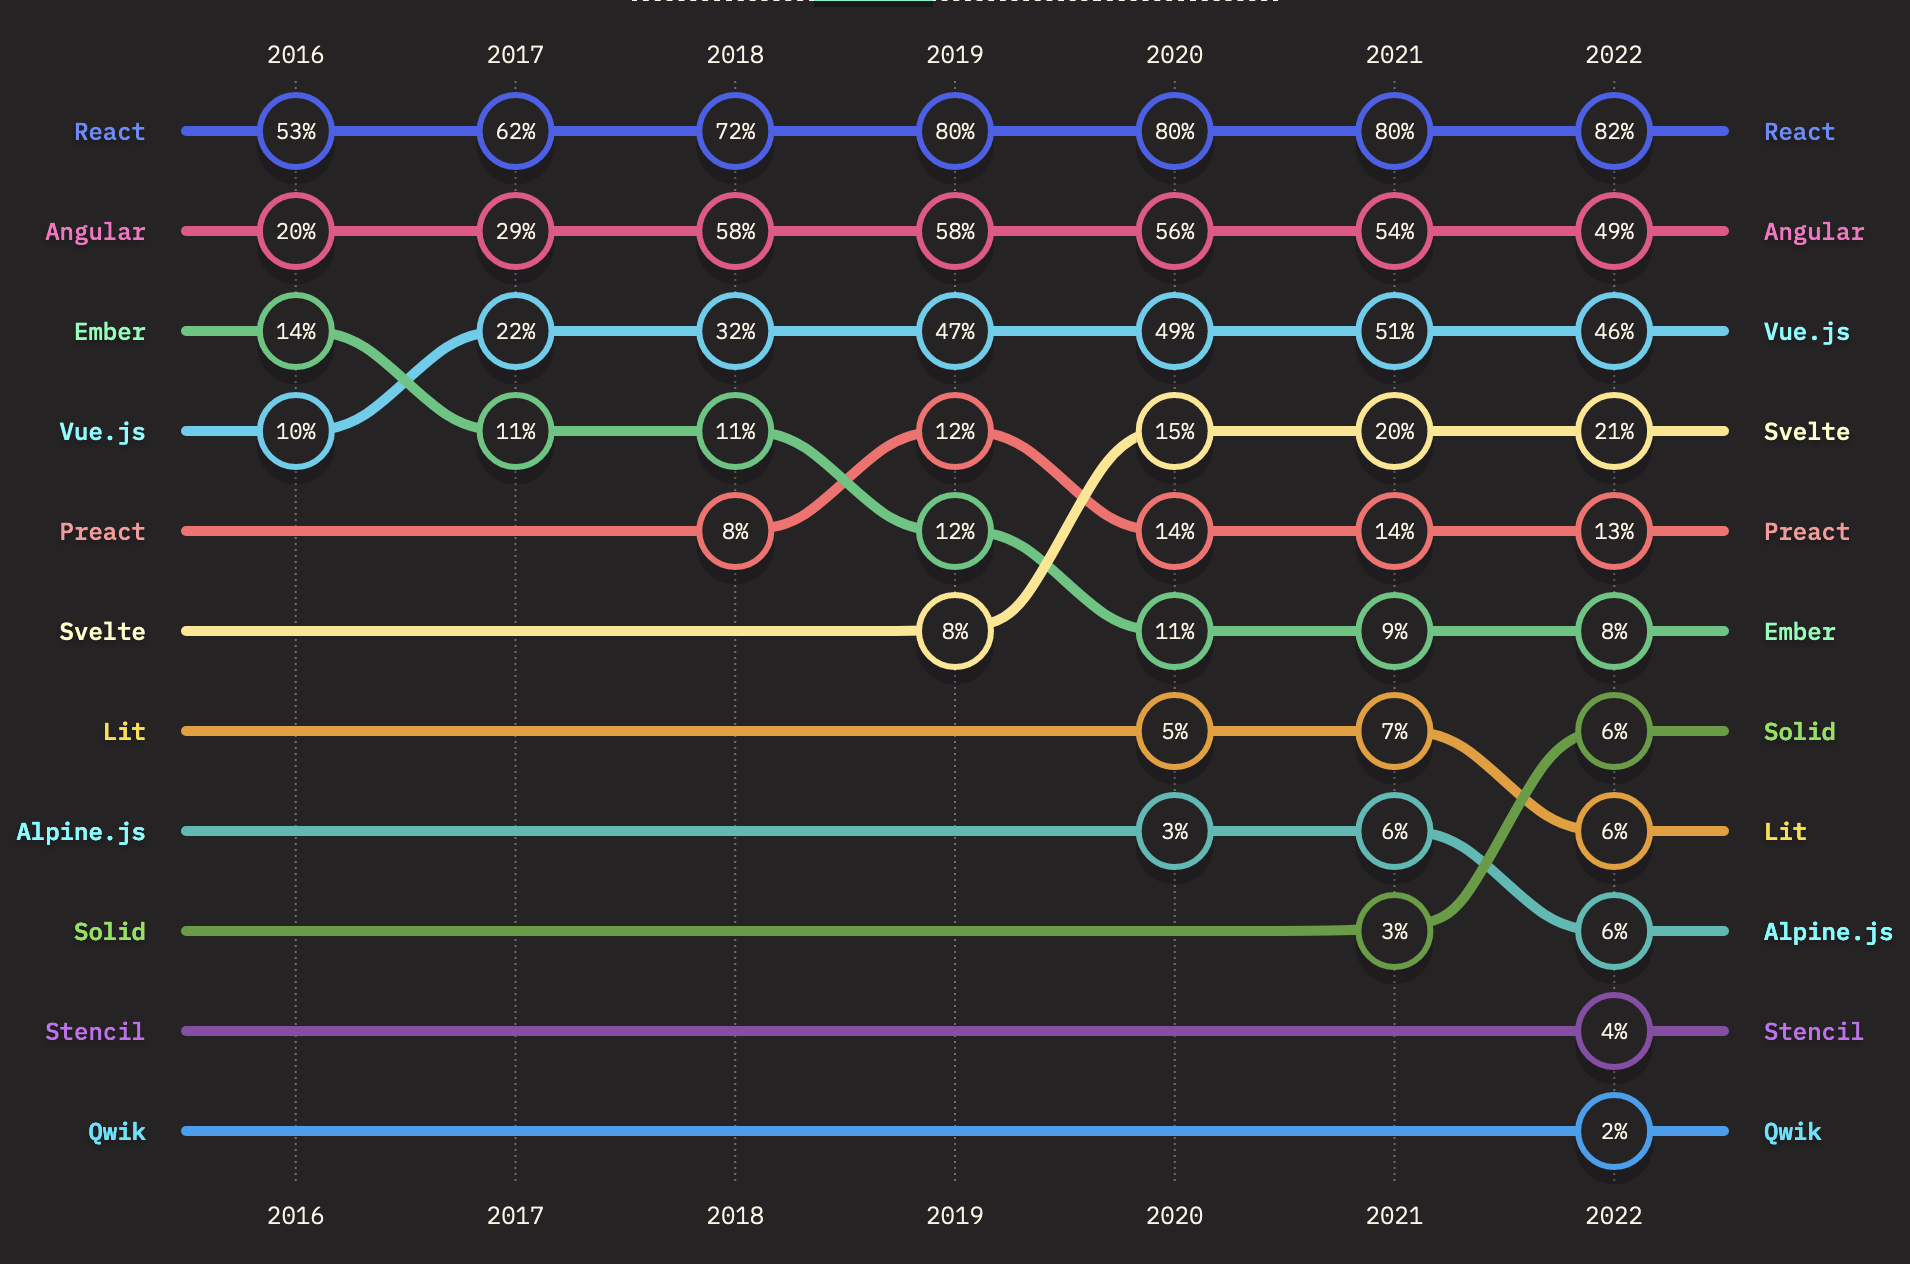
\includegraphics[scale=0.4]{04_Artefakte/01_Abbildungen/stateofjs-usage-frontend-frameworks-2022}
    \caption[{Most used frontend frameworks in 2022}]{State of JS: Most used frontend frameworks in 2022\protect\footnotemark}
    \label{fig:mostUsedFrameworks}
\end{figure}
\footnotetext{\cite{mostUsedFrontendFrameworks22}}

\subsection{React}

\emph{React} (\url{https://react.dev/}), developed by \emph{Facebook} and maintained by its successor \emph{Meta}, has become the most widely used tool for building \ac{SPA}s and is steadily leading the rankings for most used frontend frameworks both in the \emph{StackOverflow} \parencite{stackOverflowPollWebFrameworks23} and the \emph{State Of JS} \parencite{mostUsedFrontendFrameworks22} polls. By definition, it is not a framework but a \ac{UI} library that builds on other extensions to support state management, routing and deployment functionality. Although it is not a framework itself, there are existing frameworks like \emph{Next.js} (\url{https://nextjs.org/}) for the web and \emph{ReactNative} (\url{https://reactnative.dev/}) for building mobile apps using native functionality. React makes use of \ac{JSX}, which allows directly mixing inline \ac{HTML} with the \ac{JS} or \ac{TS} code structure.

\subsection{Vue.js}

\emph{Vue.js} (\url{https://vuejs.org/}) was developed by Evan You and is maintained by an international team of individuals. It had a relatively marginal presence in the US and Europe in the first years after its inception. This can be partially attributed to its origin in China, as most of its supporting modules were localised in Chinese. Over the years, it grew in popularity and received much more international support, eventually overcoming the language barrier. Unlike \emph{React}, it is billed as a "progressive framework" that provides fundamental functionality for building reactive components but also accommodates more complex use-cases \parencite{vueProgressiveFramework}. \emph{Vue.js} builds on standard \ac{JS} or \ac{TS}, \ac{HTML} and \ac{CSS} to build components, recommending a simple template mechanism mixed with reactive substitutions. However, it also supports using \ac{JSX} for specifying inline \ac{HTML} within \ac{JS}. As with \emph{React}, there are extensions and frameworks like \emph{Quasar} (\url{https://quasar.dev/}) and \emph{Nuxt} (\url{https://nuxt.com/}) that enable even more sophisticated workflows for application development and deployment.

\subsection{Angular}

\emph{Angular} was initially released by \emph{Google} in 2010 as \emph{AngularJS}  and officially discontinued in 2022 (\url{https://angularjs.org/}). A completely overhauled and currently used version 2 was released in 2016 and maintained by \emph{Google}. It is different from \emph{React} and \emph{Vue.js} in that it is a complete framework that contains everything required to build and deploy an application, and it explicitly recommends \ac{TS} as a programming language. The framework is also less flexible in that it is opinionated and has its own set of best practices baked into the framework's structure.




\section{Backend Libraries}

\subsection{Express}

The Express JS framework provides the basic functionality to create web servers including routing and middleware functionality. It was developed by TJ Holowaychuk, then sold to StrongLoop, which was subsequently acquired by IBM. It is currently under the stewardship of the OpenJS Foundation.

Express has become the de facto standard for building web services in JS, leading the ranking in the State of JS survey \parencite{mostUsedBackendFrameworks22}. Although it contains the necessary parts to build a web service, it does not enforce a specific architecture, which can be a problem for maintaining a robust application structure. For developers who prefer a more explicit structure, there are various other frameworks building on top of it and adding more opinionated structure or extensions.

\subsection{Koa}

Billed as a successor to Express, Koa is developed by the team behind Express. It aims to provide a more robust and minimalistic iteration on the middleware-based architecture of Express. Like Express, it allows for building a service from scratch in completely free form, but is also the basis for other, more explicitly structured frameworks.


\section{Backend Frameworks}

For more complex applications a more stringent and structured application structure, other frameworks might be more desirable. There are numerous \ac{JS} frameworks, some based on Express or Koa, others provide their own basis for routing. To review all possible options is beyond the scope of this study. In the following, three frameworks are selected for their specific nature related to popularity, stability but also with an explicit focus on real-time applications.

\begin{table}[ht]
\centering
\caption{State of JS survey: Most used backend frameworks \parencite{mostUsedBackendFrameworks22}}
\label{tab:backendFrameworksRanking}
\begin{tabular}[t]{lcc}
\toprule
Framework & \% of question respondents\\
\midrule
Nest & 30.2\\
Feathers & 8.8\\
Meteor & 2.7\\
\bottomrule
\end{tabular}
\end{table}


\subsection{Nest JS}

Nest JS is a backend framework for developers who look for a more strictly opinionated and robust setup than Express, e.g. for enterprise applications. It follows a modular concept, making dependencies available to the services via injection, there are multiple database options and transports can be both HTTP and WebSockets. There are \ac{CLI} scripts that enable automatic generation of boilerplate application code and the language used to build Nest applications is TypeScript. It scores the second rank among the most-used backend frameworks in the State of JS survey \parencite{mostUsedBackendFrameworks22}.

\subsection{Feathers}

This framework takes a very different approach in that it makes very little assumptions about the specific application structure. It uses aspect-oriented programming and uses a service-centric architecture. The usage of before-, after- and around-hooks (so called \textquote{cross-cutting concerns}) for the services that modify basic behaviour or add functionality. There are adapters for a wide range of databases and authentication methods. The framework has a dedicated concept of channels that enable real-time functionality and messaging to clients. Real-time transports are also abstracted and can be deployed using various different WebSockets libraries. It also provides a \ac{CLI} to generate application code that can be written in \ac{JS} or \ac{TS}.

Feathers started as a hobby project by David Luecke and Eric Kryski in 2013 \parencite{feathersFrameworkHistory} and is currently maintained by David Luecke and a community of individual contributors. In the State of JS survey, it is still in the lower percentages, but almost doubled that percentage from the previous survey in 2021 \parencite{mostUsedBackendFrameworks21}.

\subsection{Meteor}

Meteor focuses explicitly on real-time applications using WebSockets. The framework is a bit of an outlier in that its core is open-source, but other parts are proprietary code. Nonetheless, it should be mentioned, because it has been around for over ten years and it uses WebSockets exclusively. It was released in 2012 by a startup company, immediately received venture capital funding by Andreesen Horowitz and was eventually sold again in 2019.

The framework primarily uses MongoDB as a database system, provides its own package manager and ecosystem, its own build system and template system based on Mustache.

\chapter{Methodology}
\label{chapter:methodology}

This feasibility study is based on three basic parts. The first is a reference implementation, providing insights on the work that is necessary to arrive at the base functionality. After the implementation is finished, a quantitative analysis of the application's functionality is made as well as a statistical overview of the time spent on development. Additionally, there is a qualitative review of the resulting codebase and a reflection on the work process.

\section{Reference Implementation}

\subsection{Choice of concepts and tools}

In order to produce a valid test subject for the proposal, the reference implementation is created according to a prior selection of tools and methods deemed appropriate for the task at hand. The selection is made from the range presented in \autoref{chapter:concepts} and \autoref{chapter:tools}.

\subsection{Application development and deployment}

The application is implemented in its entirety, documented and packaged. Appropriate test coverage is provided and the overall time spent is logged in timesheets, categorised by the general areas of work. The application's server components are deployed to university hardware and made available over the internet. The client application is then run on a variety of different consumer computer systems.

\section{Quantitative Analysis}

\subsection{Performance Testing}

The application's performance is only tested in regard to the load put on the \ac{CPU} (server and client) as well as the network throughput and latency. It is verified that all signal processing performs as planned both through unit testing and simple testing tasks performed on the application itself. A practical test using real performers and dance interaction is beyond the scope of this feasibility study.

\subsection{Time spent}

A statistical analysis of the timesheets provides insight on the time spent on various aspects of the software. It should differentiate between basic boilerplate code that can be reused as is and custom code that is used for the actual use-case.

\section{Qualitative Analysis}

\subsection{Code Quality}

The code quality is mainly assessed in terms of volume (lines of code), complexity (number of classes and functions, cognitive complexity) and stylistic coherence.

\subsection{Critical reflection}

A critical analysis of the development process should weigh the expectations against the experiences made during implementation of the decisions made in planning the application. It should provide a critical evaluation of the feasibility and a discussion of benefits and drawbacks of establishing a task-specific application from scratch.

\chapter{Implementation}
\label{ch:implementation}

\section{Project Setup}
\label{sec:project-setup}

The underlying \emph{server infrastructure} for the reference implementation was an existing server with 16 \ac{CPU}-cores (with multithreading), 64 \ac{GB} \ac{RAM} and a 512 \ac{GB} \ac{SSD} drive, located on the \ac{JGU} campus and connected to the internet via a dedicated one-gigabit network connection.
The orchestration was deployed first to allow development on a working remote WebRTC infrastructure.
The basis was a clean, freshly bootstrapped Kubernetes installation running on the bare-metal server.
LiveKit and its Redis database were installed via the application deployment manager Helm, using an official installation chart published by its maintainers\footnote{\url{https://github.com/livekit/livekit-helm}}.
To simplify the deployment, LiveKit was placed behind the reverse proxy Traefik\footnote{\url{https://traefik.io/}} to manage \ac{SSL} termination via the LetsEncrypt\footnote{\url{https://letsencrypt.org/}} service and routing to the actual service running inside the cluster.
However, this simplified setup required LiveKit to be configured to listen on a single \ac{TCP} port instead of a range of UDP ports, as it would usually be deployed.
The potential downside of this deployment configuration was deemed insignificant since the server only needs to service a handful of users.
The detailed Kubernetes setup instructions are documented in the according folder in the project\textquotesingle s repository\footnote{Kubernetes setup instructions: \href{https://github.com/dasantonym/sensorama/tree/master/kubernetes}{https://github.com/dasantonym/sensorama/tree/master/kubernetes}}.

The \emph{LiveKit} installation was deployed with only a slight deviation from the default configuration.
It was set up to use \ac{TCP} as a transport protocol to allow easier integration with \ac{SSL} termination using the reverse proxy.
Otherwise, the configuration defined the endpoints for sending webhook requests and custom credentials for making requests to it via the server-side \ac{SDK} and generating valid access tokens for users to connect to rooms.
The Helm installation chart was used to set up the system along with its Redis database installation in a single command, and the server was immediately ready for connections.

The development process was conducted in a desktop environment, using the suite of tools developed by JetBrains (WebStorm, PyCharm and CLion), as these are free for educational use and provide a complete environment for development, including debugging, intelligent code completion, versioning, containerisation and deployment.
A local Docker Desktop installation allowed running services and databases locally to support development before publishing to the production environment.
Versioning was done via Git on the GitLab platform provided by the \ac{JGU}\footnote{\url{https://gitlab.rlp.net}}.

\section{API server}
\label{sec:api-server}

The first custom implementation, the \ac{API} server, was generated using the Feathers \ac{CLI} tool with standard username and password authentication and WebSockets, as well as \ac{HTTP} transports, enabled.
It provides the core services for Users, Spaces, Tokens and LiveKit events.
These services were autogenerated using the Feathers \ac{CLI} utility.
They were used largely unmodified, except for adding the properties on the models for Users and Spaces as defined in \autoref{sec:datamodeling}.
A custom service class was added for the Tokens, as these do not persist in the database and instead are generated on the fly by the LiveKit server \ac{SDK}.
All other boilerplate code for the \ac{API}, including the MongoDB integration, the authentication mechanism, and the REST and WebSockets transport integrations, were also autogenerated using the \ac{CLI}.
An additional custom Livekit event service was added to the API, allowing it to receive webhook requests via \ac{HTTP} from the LiveKit server containing updates on connecting and disconnecting users.
These events do not persist in the database but are relayed instead to the connected users via the real-time channels.
The channels feature provided by Feathers was used to automatically subscribe, connecting users to updates on the services for Spaces and Livekit events.

\section{Core SDK}
\label{sec:core-sdk}

The basic functionality was bundled in an \ac{NPM} module to make the base code independent of the use case, which could later be used in other projects.
This module contains the abstract classes \textquote{DataProducer}, \textquote{HeadTracker} and \textquote{SonificationController} alongside the message specification for the various types of transmitted data.
It was written to propagate updates via events instead of the reactive patterns used in Vue so that it can also be used independently from the framework used for the study.
Unit tests were added to the module to maintain a stable implementation.

\section{User interface}
\label{sec:user-interface}

The Quasar framework provides a \ac{CLI} to generate new projects, which allows selecting basic implementation details (e.g.\ language, state management) and producing a complete and working empty Vue project with sample components that served as the starting point for the \ac{UI} implementation.
The first thing added to the project was the library \textquote{feathers-pinia}\footnote{\url{https://feathers-pinia.pages.dev}}, which is provided by the Feathers developer community and promises easy integration of an existing Feathers \ac{API} with any Vue project using the Pinia\footnote{\url{https://pinia.vuejs.org/}} state management system used by Vue.
The extension was integrated by linking the client library that the Feathers server project automatically generates by referencing the \ac{API}\textquotesingle s project folder and configuring basic authentication settings.
The routing configuration and page components were set up according to the sitemap (see !!!autoref{fig:sitemap}).

The overview page for the spaces presents a list of the names alongside the currently connected users and buttons to either join as a participant or passively view it as a spectator.
On joining a space, the user first needs to activate their microphone to activate the audio context.
The user is then presented with three basic control panels.
The \textquote{Data producer} panel allows setting a URL of a local WebSockets server published by a data producer, setting the message type received from it, and optionally enabling a tracing function to log the packet transmission statistics.
Once connected, the panel shows a preview of the incoming points data, transmission statistics and a button to disconnect.
Internally, the panel creates a reactive data store that instantiates the \textquote{DataProducer} class from the core \ac{SDK}, watches incoming message events and populates the received data as reactive properties to be used across the \ac{UI} in various other components without the need of creating additional class instances.
The second panel, \textquote{Head tracker}, works similarly but uses the Web Bluetooth \ac{API} to select a nearby device and connect to it to receive its data messages.
The third component configures the sonification by setting thresholds on incoming movement quality values.
It connects to an instance of the \textquote{SonificationController} class from the core \ac{SDK} and allows the configuration of event thresholds, sound selection and tonal configuration.

When using the page to view a space, there is only one component, the \textquote{SpaceViewer}, that shows a \ac{3D} room in which all incoming points are rendered as small spheres, giving the impression of a human figure.
For each participant, there is a differently coloured light source that follows the centre of mass of the points associated with the participant.
The viewer also renders all sonifications and audio streams at their respective spatial positions.
This allows the user to view the \ac{3D} scene on screen while listening to binaural audio or to use the built-in \ac{VR} functionality to experience the scene in a visually immersive way.

\section{Data producers}
\label{sec:data-producers}

The general \emph{data producer} was written in Python and provides multiple data sources: an interface to a Blazepose implementation on the Oak-D \ac{3D} camera, as well as reading depth images as point clouds from the camera and an interface to load and playback motion capture data in the \ac{BVH} file format.
All three data sources were implemented as separate Python classes because the classes related to the Oak-D camera were built by modifying existing code for pose recognition~\parencite{githubDepthAiBlazePose} and point cloud processing~\parencite{githubDepthAiPointcloud}.
The \ac{BVH} data source was created from scratch and implemented to facilitate testing and development by using playback of motion capture data of professional dancers pre-recorded on the Captury Live system.
All data source classes were set up to support calling a function in a loop and returning current point data as a multidimensional array.
The returned data is packed as a byte sequence and sent over WebSockets in the appropriate format (see \autoref{sec:datamodeling}).
This way, the disparate sources could be imported into a single central file that uses a combined set of utility functions for running a WebSockets server and packing data.
Due to the lack of a Python-based client for the Captury Live system, the Captury producer had to be implemented separately as a C++ project using CMake\footnote{\url{https://cmake.org/}} as a build system and based on the \textquote{RemoteCaptury} client library~\parencite{githubRemoteCaptury}, as well as an example project for a WebSockets server implementation in C++~\parencite{githubCppWebSocketsDemo}.

The custom-built head-tracking device was implemented as an Arduino project.
As such, it was first realised as a hardware setup and then outfitted with custom firmware written in the Arduino-specific flavour of C/C+.
The hardware implementation was created using the \textquote{Arduino Connect RP2040}\footnote{\url{https://docs.arduino.cc/hardware/nano-rp2040-connect/}}, which is based on the Raspberry PI 2040 microcontroller and has an onboard BluetoohLE module.
The \ac{IMU} module used was the \textquote{9-DOF Absolute Orientation IMU Fusion Breakout}\footnote{\url{https://www.adafruit.com/product/4646}} which uses the BNO055\footnote{\url{https://www.bosch-sensortec.com/products/smart-sensor-systems/bno055/}} chip produced by Bosch.
This chip has the benefit of already pre-processing the data from the gyroscope, accelerometer and magnetometer into an absolute world position that can be directly read from the breakout board via the \ac{I2C} bus.
As a third component, a small 3.7V lithium battery was added alongside a charging module\footnote{\url{https://www.adafruit.com/product/1905}}.
Only six connections needed to be soldered between the three modules (2x charger and 4x \ac{IMU}), and the resulting circuit was ready to function as a custom head tracker.
For the software implementation, the basic example code for the Adafruit module was used to set up continuous polling of the positioning module, reading the values for position and device calibration status and sending them as byte sequences at a fixed rate of ~25fps over BluetoothLE\@.

\chapter{Conclusion}

\section{Evaluation results}

\section{Critical reflection}

\section{Outlook}



\pagenumbering{Roman}

\setcounter{page}{\value{romanConsecutive}-1} % decrease counter by one 
\printbibliography[title={Bibliography}]
% Erklärender Text zu dieser Datei --------------------------------------------------------
% Die Datei 01_Anhang.tex dient der Definition des Anhangs und dessen Reihenfolge.
% -----------------------------------------------------------------------------------------
\appendix
\clearpage
\pdfbookmark{Appendix}{appendix}
\chapter{Appendix}

% Anhang nachfolgend einfügen ----------------------------------------------------------------------

%\begin{longlisting}
%\label{app:longlisting}
%\caption{Langes Listing in Java}
%\label{listing:longlisting}
%\inputminted{java}{04_Artefakte/03_Listings/Daten.java}
%\end{longlisting}
%
%\chapter{Anhang Auszug PDF}
%\label{app:auszugPDF}
%\begin{figure}[h]
%    \centering
%    \frame{\includegraphics[width=0.7\linewidth]{04_Artefakte/BeispielPDF.pdf}}
%    \caption[Beispiel für den Auszug aus einer PDF]{Beispiel für den Auszug aus einer PDF im Anhang}
%\end{figure}
%
%\chapter{Anhang Tabelle}
%\label{app:longtable}
%\input{04_Artefakte/02_Tabellen/LongSample}


\usestandardtocs
\bookmarksetup{startatroot}% siehe bookmark-Anleitung

\end{document}
